
\UseRawInputEncoding
\documentclass[12pt,letterpaper]{article}

% --- Paquetes requeridos ---
\usepackage[utf8]{inputenc}
\usepackage[spanish,es-nodecimaldot]{babel}
\usepackage{geometry}
\geometry{top=2.54cm, bottom=2.54cm, left=2.54cm, right=2.54cm}
\usepackage{setspace}
\onehalfspacing % Espaciado de 1.5 para lecturas técnicas (formato APA permite adaptaciones)
\usepackage{times} % Tipografía Times New Roman
\usepackage{indentfirst} % Indentación en el primer párrafo de cada sección
\usepackage{titlesec}
\usepackage{xcolor}
\usepackage{listings}
\usepackage{hyperref}
\usepackage{biblatex}
\usepackage{fancyhdr}
\usepackage{amsmath}
\usepackage{graphicx}
\graphicspath{{images/}{docs/images/}{fiis/docs/images/}}
\usepackage{hanging}

% --- Configuración de hipervínculos ---
\hypersetup{
    colorlinks=true,
    linkcolor=black,
    filecolor=blue,      
    urlcolor=blue,
    citecolor=black
}

% --- Formato de títulos estilo APA 7 ---
\titleformat{\section}{\normalfont\fontsize{12}{14}\bfseries\filcenter}{\thesection. }{0em}{}
\titleformat{\subsection}{\normalfont\fontsize{12}{14}\bfseries}{\thesubsection. }{0em}{}
\titleformat{\subsubsection}{\normalfont\fontsize{12}{14}\bfseries\itshape}{\thesubsubsection. }{0em}{}

% --- Configuración de Listings para bloques de código ---
\definecolor{codegray}{rgb}{0.95,0.95,0.95}
\definecolor{codeblue}{rgb}{0.1,0.1,0.6}
\definecolor{codegreen}{rgb}{0.1,0.5,0.1}

\lstset{
    backgroundcolor=\color{codegray},
    basicstyle=\ttfamily\small,
    breakatwhitespace=false,
    breaklines=true,
    captionpos=b,
    commentstyle=\color{codegreen},
    keywordstyle=\color{codeblue}\bfseries,
    numbers=left,
    numberstyle=\tiny\color{gray},
    numbersep=5pt,
    showspaces=false,
    showstringspaces=false,
    showtabs=false,
    stringstyle=\color{purple},
    tabsize=4,
    frame=single,
    rulecolor=\color{gray},
    language=Java
}

% --- Encabezado y pie de página ---
\pagestyle{fancy}
\fancyhf{}
\rhead{\thepage}
\lhead{Documentación del Módulo de Autenticación y Usuarios - SGI-FIIS}
\renewcommand{\headrulewidth}{0.5pt}

% --- Inicio del documento ---
\begin{document}

% --- PORTADA ---
\begin{titlepage}
    \begin{center}
        \vspace*{1cm}
        
        \large
        \textbf{UNIVERSIDAD NACIONAL AGRARIA DE LA SELVA}\\
        \textbf{FACULTAD DE INGENIERÍA EN INFORMÁTICA Y SISTEMAS}\\
        
        \vspace*{2cm}
        
        \Large
        \textbf{DISEÑO E IMPLEMENTACIÓN DEL MÓDULO DE AUTENTICACIÓN Y GESTIÓN DE USUARIOS BAJO ARQUITECTURA LIMPIA PARA EL SISTEMA DE GESTIÓN DE INVESTIGACIÓN DE LA FIIS (SGI-FIIS)}\\
        
        \vspace*{2.5cm}
        
        \large
        \textbf{Documento de Especificación Técnica e Implementación}\\
        
        \vspace*{2cm}
        
        \textbf{Autor:}\\
        Equipo SGI-FIIS\\
        
        \vspace*{1.5cm}
        
        \textbf{Curso/Proyecto:}\\
        Construcción de software II\\
        
        \vspace*{2cm}
        
        \textbf{Tingo María, Perú}\\
        \textbf{2026}
    \end{center}
\end{titlepage}

\newpage

% --- RESUMEN ---
\section*{Resumen}
El presente documento describe el diseño, la arquitectura y el proceso de implementación del módulo de Autenticación y Gestión de Usuarios para el Sistema de Gestión de Investigación de la Facultad de Ingeniería en Informática y Sistemas (SGI-FIIS). Este módulo constituye la base de seguridad y autorización del sistema, posibilitando el control de acceso de todos los actores involucrados en la investigación de la facultad (estudiantes, docentes, coordinadores, directores, decanos y administradores). La implementación técnica se ha desarrollado utilizando la plataforma Java con el framework Spring Boot, adoptando un diseño arquitectónico basado en la Arquitectura Limpia (Clean Architecture) para separar rigurosamente las reglas de negocio de la infraestructura tecnológica. Asimismo, el módulo integra autenticación local por medio de JSON Web Tokens (JWT) y un mecanismo seguro de auto-registro con verificación por código enviado a la bandeja de correo institucional, garantizando un registro controlado y un inicio de sesión seguro. La persistencia de datos se realiza en un motor PostgreSQL mediante Spring Data JPA, utilizando migraciones versionadas con la herramienta Flyway.

\textbf{Palabras clave:} Autenticación, Gestión de Usuarios, JWT, Auto-registro, Clean Architecture, Spring Boot, PostgreSQL, Flyway.

\newpage

% --- INTRODUCCIÓN ---
\section{Introducción}
El desarrollo científico y la gestión académica en las facultades de ingeniería demandan herramientas informáticas que automaticen los procesos de registro, evaluación y seguimiento de proyectos, tesis y publicaciones. El Sistema de Gestión de Investigación de la Facultad de Ingeniería en Informática y Sistemas (SGI-FIIS) ha sido concebido para cubrir esta necesidad. Sin embargo, para que un sistema administrativo de esta envergadura funcione adecuadamente, es imperativo contar con un sólido sistema de control de acceso y seguridad.

El módulo de Autenticación y Gestión de Usuarios representa la piedra angular de esta plataforma. Su objetivo fundamental es asegurar que cada usuario que interactúe con el sistema posea una identidad digital verificada y los permisos estrictamente necesarios para desempeñar su función. A través de este módulo se controlan las operaciones críticas de registro de investigadores, validación de credenciales institucionales, auto-registro de estudiantes mediante validación por correo electrónico institucional y el control de accesos basados en roles.

\subsection{Objetivos del Módulo}
El desarrollo del módulo persigue dos objetivos centrales. Por un lado, busca automatizar la administración del ciclo de vida de los usuarios dentro del sistema, permitiendo su registro, edición, desactivación temporal y el reinicio de credenciales. Por otro lado, busca proveer un mecanismo seguro y controlado de auto-registro por correo para la comunidad estudiantil, permitiéndoles crear sus propias cuentas de manera autónoma y segura.

\subsection{Justificación de la Solución}
La elección de integrar tanto el registro por administración centralizada como el auto-registro guiado por verificación de correo institucional responde a la diversidad de usuarios finales del sistema. Mientras que el personal administrativo y los docentes de investigación se gestionan administrativamente, los estudiantes y tesistas pueden auto-registrarse de manera ágil utilizando sus cuentas institucionales verificadas por código en un proceso en dos pasos.

\newpage

% --- MARCO ARQUITECTÓNICO ---
\section{Arquitectura del Sistema (Clean Architecture)}
Para garantizar la mantenibilidad, escalabilidad y testabilidad del sistema, se adoptó el patrón de diseño arquitectónico de Arquitectura Limpia (Clean Architecture). Este enfoque promueve un desacoplamiento estricto de las reglas de negocio respecto a los frameworks, bases de datos y detalles de infraestructura. La regla fundamental de este diseño establece que las dependencias deben apuntar únicamente hacia adentro, es decir, el núcleo del dominio no debe conocer ningún detalle de las capas externas.

\subsection{Estructura del Proyecto y Capas}
El backend del SGI-FIIS se divide en cuatro capas claramente delimitadas, estructuradas de la siguiente manera dentro del paquete de cada módulo:
\begin{enumerate}
    \item \textbf{Capa de Dominio (Domain):} Es el núcleo del sistema. Contiene los modelos de negocio puros, los objetos de valor, los eventos del dominio y los puertos (interfaces) que definen cómo el dominio interactúa con el mundo exterior. Esta capa es completamente independiente de Spring Boot, JPA, bases de datos o cualquier librería de terceros.
    \item \textbf{Capa de Aplicación (Application):} Contiene la lógica específica de la aplicación y la orquestación de los casos de uso. En ella se implementan los servicios que ejecutan flujos de negocio específicos, manipulando las entidades de dominio y comunicándose con las interfaces definidas en la capa de dominio.
    \item \textbf{Capa de Infraestructura (Infrastructure):} Contiene la implementación de los detalles tecnológicos. Incluye la persistencia física (entidades JPA, repositorios Spring Data, adaptadores de bases de datos), la seguridad web (configuración de Spring Security, filtros JWT, handlers OAuth2) y la integración de servicios de terceros.
    \item \textbf{Capa de Presentación (Presentation):} Actúa como la interfaz de comunicación con los clientes externos. Contiene los controladores REST encargados de recibir las peticiones HTTP, validar sintácticamente los datos de entrada, invocar los casos de uso correspondientes y retornar las respuestas adecuadas por medio de objetos de transferencia de datos (DTO).
\end{enumerate}

El desacoplamiento de capas permite realizar pruebas unitarias sobre los casos de uso del sistema sin necesidad de levantar bases de datos reales o servidores web. La persistencia se inyecta en los casos de uso mediante la inversión de dependencias: la aplicación consume las interfaces (puertos) del dominio, y la infraestructura implementa dichas interfaces (adaptadores).

Esta organización y el flujo de dependencias unidireccional hacia el núcleo del dominio se representa de forma visual en la Figura~\ref{fig:arquitectura_capas}.

\begin{figure}[htbp]
    \centering
    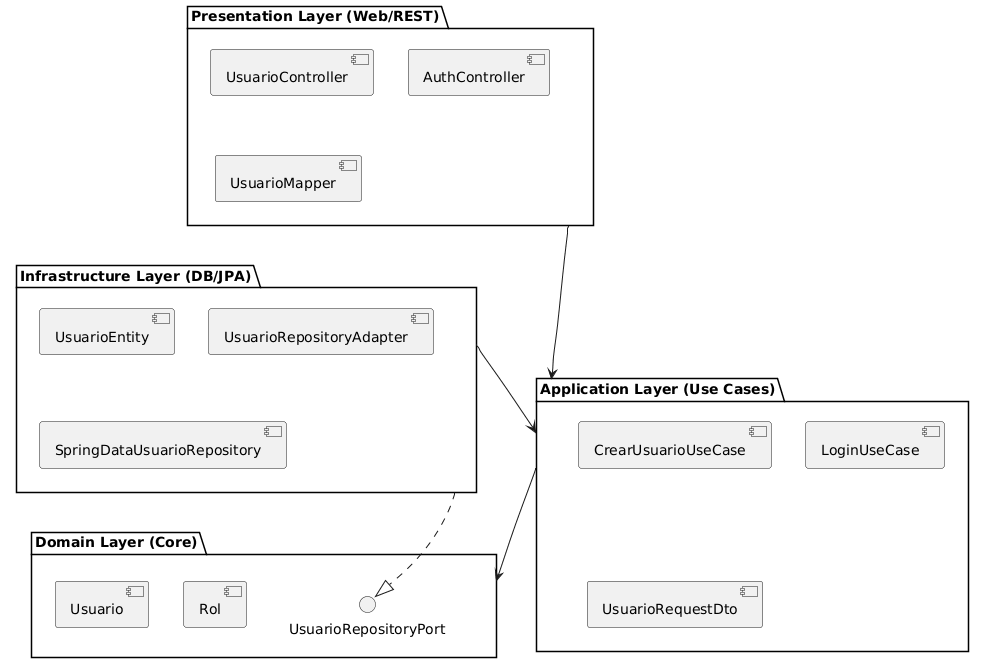
\includegraphics[width=0.85\textwidth]{arquitectura_capas}
    \caption{Arquitectura en capas y flujo de dependencias del módulo de usuarios.}
    \label{fig:arquitectura_capas}
\end{figure}

\subsection{Arquitectura de Despliegue e Infraestructura}
Para garantizar que la aplicación backend sea fácilmente desplegable en entornos de staging y producción, el sistema se encuentra completamente contenedorizado mediante Docker y orquestado a través de Docker Compose. La infraestructura lógica del módulo se compone de cuatro nodos fundamentales: el navegador del cliente (Frontend Web), el servicio de backend Spring Boot empaquetado, la base de datos PostgreSQL y el servidor SMTP de correo para el envío de códigos de verificación.

Esta distribución física de componentes y los flujos de comunicación a través de HTTPS/REST, JDBC y protocolos de autenticación se detalla en la Figura~\ref{fig:arquitectura_despliegue}.

\begin{figure}[htbp]
    \centering
    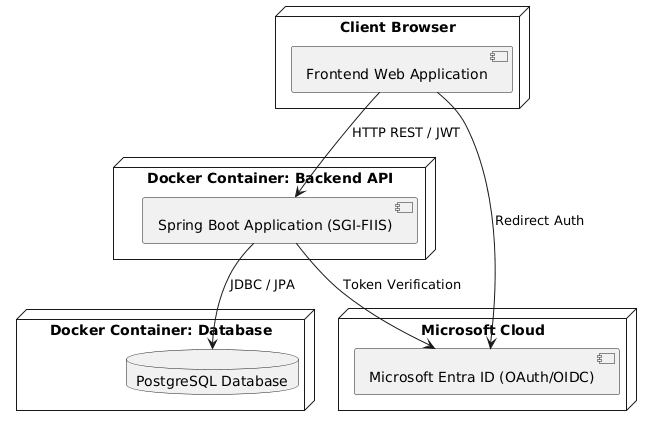
\includegraphics[width=0.85\textwidth]{arquitectura_despliegue}
    \caption{Diagrama de arquitectura de despliegue y flujo de integración física del sistema.}
    \label{fig:arquitectura_despliegue}
\end{figure}

\newpage

% --- MODELO DE DATOS ---
\section{Modelo de Datos y Persistencia}
La base de datos relacional PostgreSQL sirve como motor de almacenamiento primario del backend de SGI-FIIS. Para estructurar y poblar el esquema del módulo de seguridad de forma consistente, se utiliza Flyway como motor de migraciones, garantizando que el diseño de las tablas se aplique idénticamente en entornos de desarrollo, pruebas y producción.

\subsection{Estructura de las Tablas}
La seguridad del sistema se fundamenta en un modelo de control de acceso basado en roles (RBAC - Role-Based Access Control) soportado por dos tablas principales:
\begin{itemize}
    \item \textbf{roles:} Almacena la definición de los diferentes perfiles autorizados en el sistema. Los roles predefinidos corresponden a: ADMIN, ESTUDIANTE, DOCENTE\_INVESTIGADOR, COORDINADOR\_GRUPO, DIRECTOR\_INVESTIGACION, DECANO y EVALUADOR.
    \item \textbf{usuarios:} Contiene la información de perfil y las credenciales de seguridad de los usuarios registrados. Soporta tanto el login tradicional mediante campos de contraseña hasheada como el campo oauth\_provider reservado para auditoría o integraciones futuras.
\end{itemize}

El campo \texttt{must\_change\_password} es un indicador booleano que obliga al usuario a actualizar su contraseña de forma mandatoria en el primer inicio de sesión. Por otro lado, la columna \texttt{oauth\_provider} puede almacenar información de proveedor externo en el caso de migraciones, aunque la autenticación actual del sistema se gestiona de manera puramente local y segura.

Las relaciones de cardinalidad, llaves primarias, llaves foráneas y tipos de datos físicos del esquema de persistencia se presentan de forma gráfica en la Figura~\ref{fig:modelo_relacional}.

\begin{figure}[htbp]
    \centering
    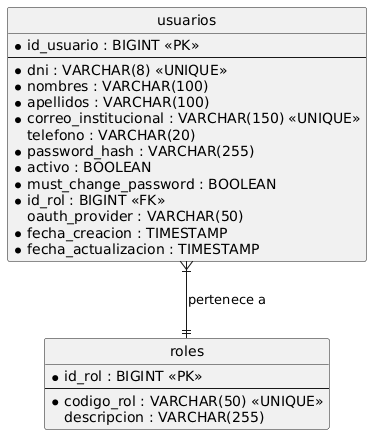
\includegraphics[width=0.65\textwidth]{modelo_relacional}
    \caption{Diagrama Entidad-Relación (DER) de las tablas de usuarios y roles del sistema SGI-FIIS.}
    \label{fig:modelo_relacional}
\end{figure}

\subsection{Script de Creación de Tablas (SQL)}
La definición física de las tablas se implementa en la migración \texttt{V1\_\_create\_roles\_and\_usuarios.sql} y la columna OAuth se añade en \texttt{V3\_\_add\_oauth\_provider\_to\_usuarios.sql}. A continuación, se presenta la estructura relacional expresada en código SQL:

\begin{lstlisting}[language=SQL, caption={Esquema físico de base de datos para roles y usuarios.}]
-- Tabla de roles del sistema
CREATE TABLE roles (
    id_rol       BIGSERIAL    PRIMARY KEY,
    codigo_rol   VARCHAR(50)  NOT NULL UNIQUE,
    descripcion  VARCHAR(255)
);

-- Tabla de usuarios del sistema
CREATE TABLE usuarios (
    id_usuario            BIGSERIAL     PRIMARY KEY,
    dni                   VARCHAR(8)    NOT NULL UNIQUE,
    nombres               VARCHAR(100)  NOT NULL,
    apellidos             VARCHAR(100)  NOT NULL,
    correo_institucional  VARCHAR(150)  NOT NULL UNIQUE,
    telefono              VARCHAR(20),
    password_hash         VARCHAR(255)  NOT NULL,
    activo                BOOLEAN       NOT NULL DEFAULT TRUE,
    must_change_password  BOOLEAN       NOT NULL DEFAULT TRUE,
    id_rol                BIGINT        NOT NULL REFERENCES roles(id_rol),
    oauth_provider        VARCHAR(50), -- null si es login local
    fecha_creacion        TIMESTAMP     NOT NULL DEFAULT NOW(),
    fecha_actualizacion   TIMESTAMP     NOT NULL DEFAULT NOW()
);

-- Indices para busquedas frecuentes
CREATE INDEX idx_usuarios_rol ON usuarios(id_rol);
CREATE INDEX idx_usuarios_activo ON usuarios(activo);
CREATE INDEX idx_usuarios_dni ON usuarios(dni);
CREATE INDEX idx_usuarios_correo ON usuarios(correo_institucional);
CREATE INDEX idx_usuarios_oauth_provider ON usuarios(oauth_provider);
\end{lstlisting}

Las restricciones de integridad aseguran la unicidad del DNI y del correo institucional, previniendo duplicidades. Los índices se han ubicado estratégicamente en las columnas más utilizadas en las cláusulas \texttt{WHERE} de las consultas internas, tales como la verificación del correo durante el login y la búsqueda de usuarios activos.

\newpage

% --- ESPECIFICACIÓN FUNCIONAL Y FLUJOS ---
\section{Especificación Funcional y Flujos de Control}
El comportamiento operativo del módulo abarca el inicio de sesión convencional con JWT, el auto-registro con verificación por código por correo, el ciclo de cambio de contraseñas y la administración general de cuentas de usuario por parte de los administradores.

Para modelar y estructurar el comportamiento del sistema, la interacción de los distintos actores con las funcionalidades de seguridad y administración se representa de forma segmentada y clara mediante diagramas de casos de uso UML específicos por cada uno de los siete roles del sistema. Esta organización individualizada previene el cruce de líneas y la sobrecarga visual en la documentación.

La Figura~\ref{fig:casos_uso_admin} ilustra las acciones de administración técnica de usuarios, líneas de investigación y membresías de grupos a cargo del Administrador.

\begin{figure}[htbp]
    \centering
    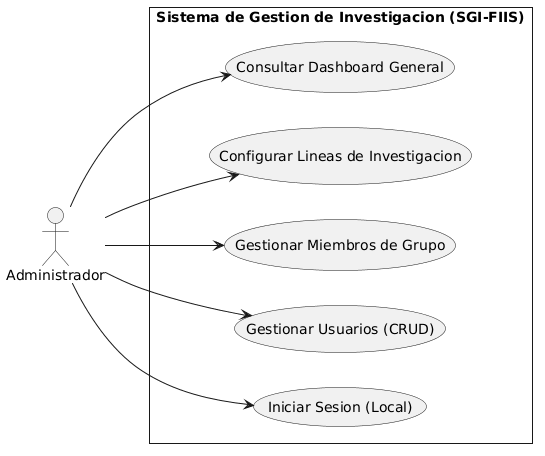
\includegraphics[width=0.85\textwidth]{casos_uso_admin}
    \caption{Diagrama de casos de uso UML para el rol de Administrador.}
    \label{fig:casos_uso_admin}
\end{figure}

Por otro lado, la interacción del Estudiante o Tesista con el auto-registro, inicio de sesión local, el registro de planes de tesis y la subsanación de observaciones se representa en la Figura~\ref{fig:casos_uso_estudiante}.

\begin{figure}[htbp]
    \centering
    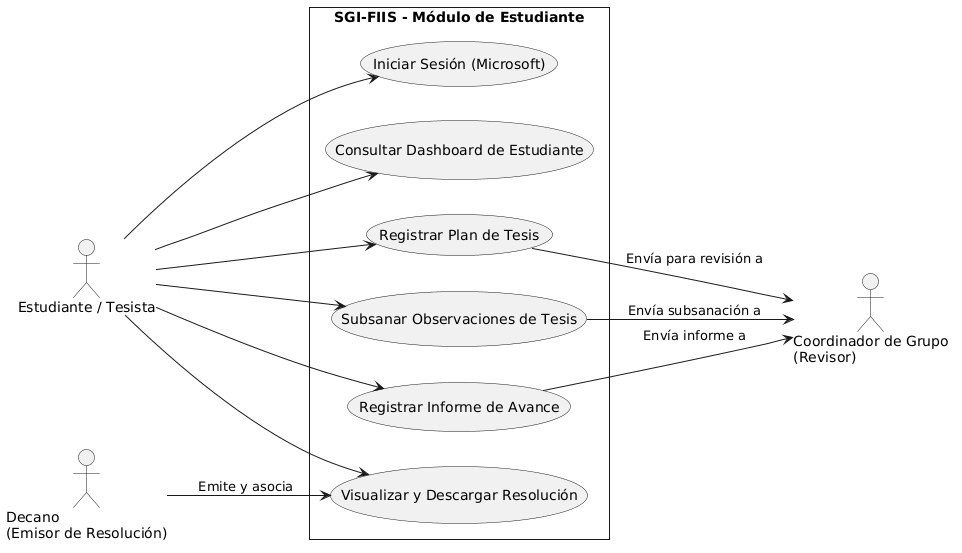
\includegraphics[width=0.85\textwidth]{casos_uso_estudiante}
    \caption{Diagrama de casos de uso UML para el rol de Estudiante / Tesista.}
    \label{fig:casos_uso_estudiante}
\end{figure}

Asimismo, las funcionalidades específicas del Docente Investigador para registrar proyectos de investigación y subsanar sus respectivas observaciones se muestran en la Figura~\ref{fig:casos_uso_docente}.

\begin{figure}[htbp]
    \centering
    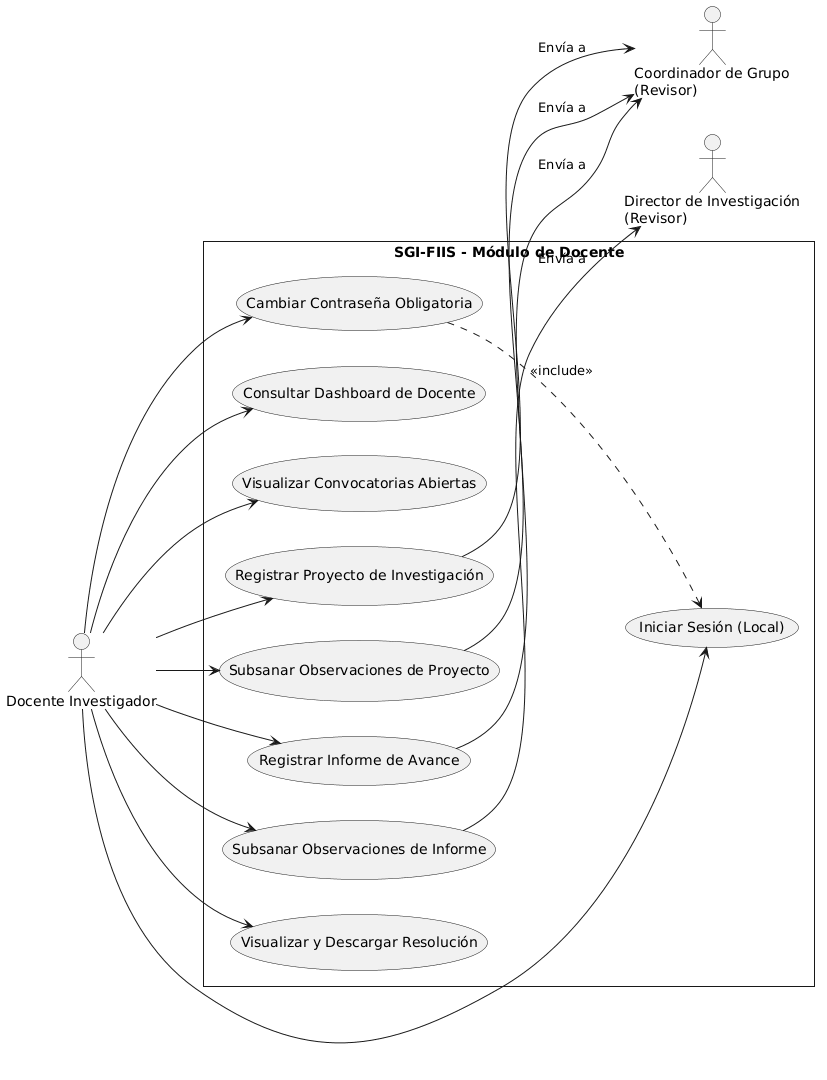
\includegraphics[width=0.85\textwidth]{casos_uso_docente}
    \caption{Diagrama de casos de uso UML para el rol de Docente Investigador.}
    \label{fig:casos_uso_docente}
\end{figure}

El flujo de revisión y control académico por parte del Coordinador de Grupo se detalla en la Figura~\ref{fig:casos_uso_coordinador}, mostrando su interacción con el Solicitante (docente o estudiante) y el Director de Investigación como siguiente revisor.

\begin{figure}[htbp]
    \centering
    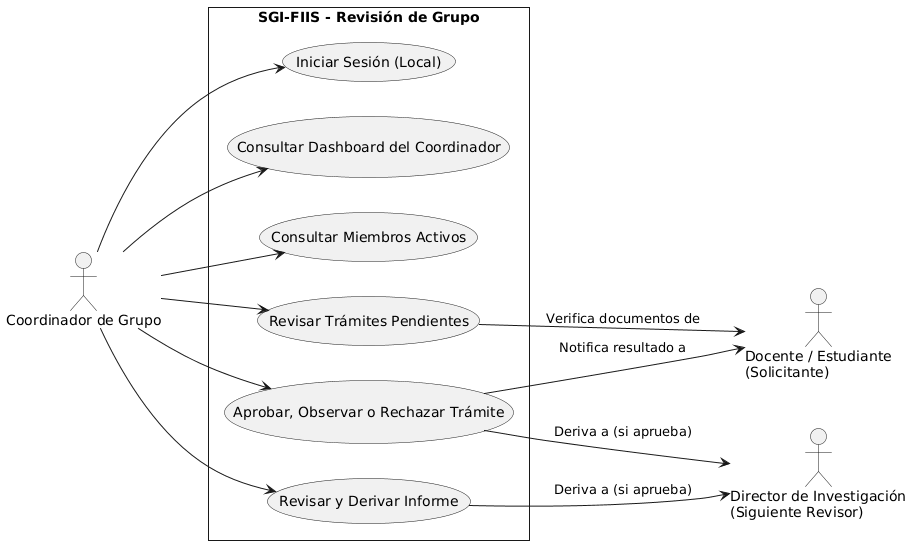
\includegraphics[width=0.85\textwidth]{casos_uso_coordinador}
    \caption{Diagrama de casos de uso UML para el rol de Coordinador de Grupo.}
    \label{fig:casos_uso_coordinador}
\end{figure}

La Figura~\ref{fig:casos_uso_director} describe las interacciones del Director de Investigación para evaluar trámites pre-revisados por el Coordinador, derivar aprobaciones al Decanato, devolver observaciones y registrar las convocatorias oficiales.

\begin{figure}[htbp]
    \centering
    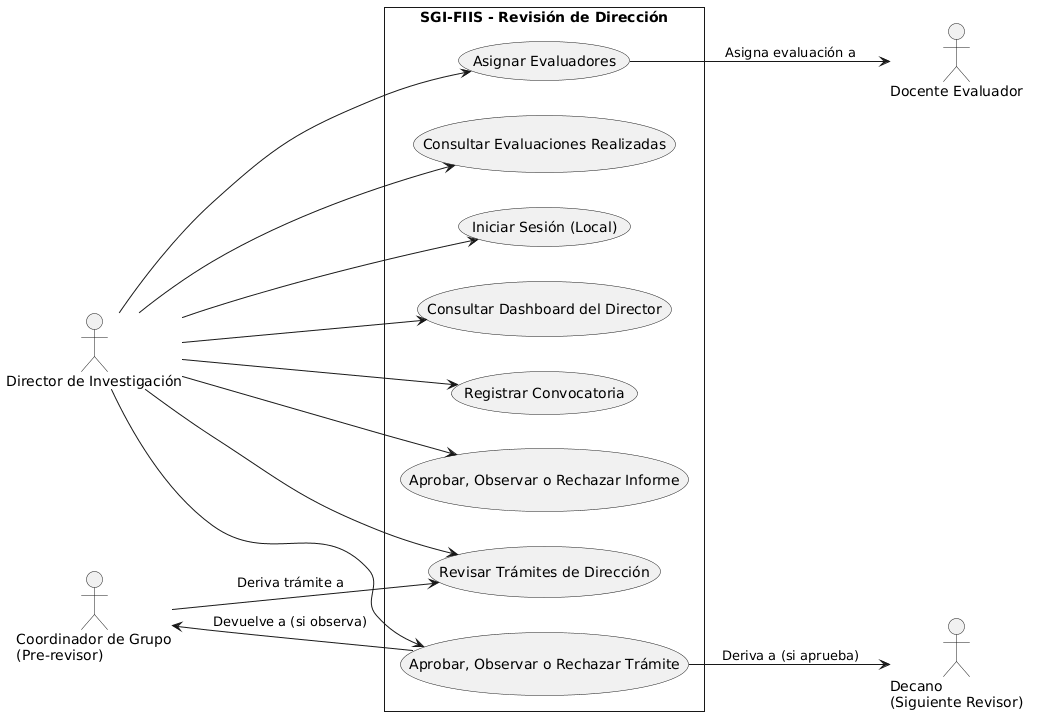
\includegraphics[width=0.85\textwidth]{casos_uso_director}
    \caption{Diagrama de casos de uso UML para el rol de Director de Investigación.}
    \label{fig:casos_uso_director}
\end{figure}

Por su parte, las acciones del Decano para revisar expedientes avalados por Dirección, registrar resoluciones académicas y formalizar la aprobación de proyectos se ilustran en la Figura~\ref{fig:casos_uso_decano}.

\begin{figure}[htbp]
    \centering
    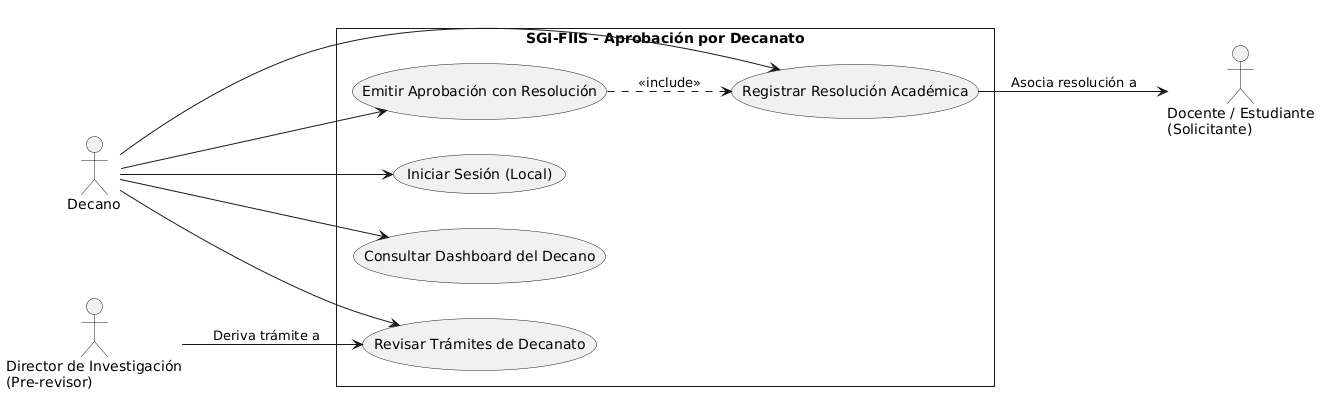
\includegraphics[width=0.85\textwidth]{casos_uso_decano}
    \caption{Diagrama de casos de uso UML para el rol de Decano.}
    \label{fig:casos_uso_decano}
\end{figure}

Finalmente, las interacciones específicas del Docente Evaluador para dictaminar los proyectos de investigación asignados por Dirección y reportar sus calificaciones se especifican en la Figura~\ref{fig:casos_uso_evaluador}.

\begin{figure}[htbp]
    \centering
    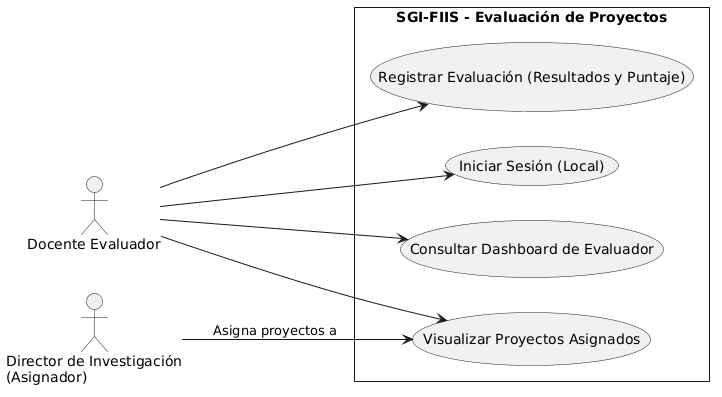
\includegraphics[width=0.85\textwidth]{casos_uso_evaluador}
    \caption{Diagrama de casos de uso UML para el rol de Docente Evaluador.}
    \label{fig:casos_uso_evaluador}
\end{figure}

\subsection{Autenticación Convencional (JWT)}
Cuando un usuario inicia sesión con correo y contraseña, el sistema valida que las credenciales coincidan con la firma hasheada (\texttt{BCrypt}) y verifica que la cuenta se encuentre activa. Si la autenticación es exitosa, se genera un token JSON Web Token (JWT) firmado digitalmente que expira tras un periodo predeterminado. El frontend debe enviar este token en el encabezado HTTP \texttt{Authorization: Bearer <token>} para cada consulta protegida subsiguiente.

El flujo operativo descrito anteriormente y las transacciones de validación de identidad correspondientes se visualizan gráficamente en el diagrama de secuencia de la Figura~\ref{fig:login_local}.

\begin{figure}[htbp]
    \centering
    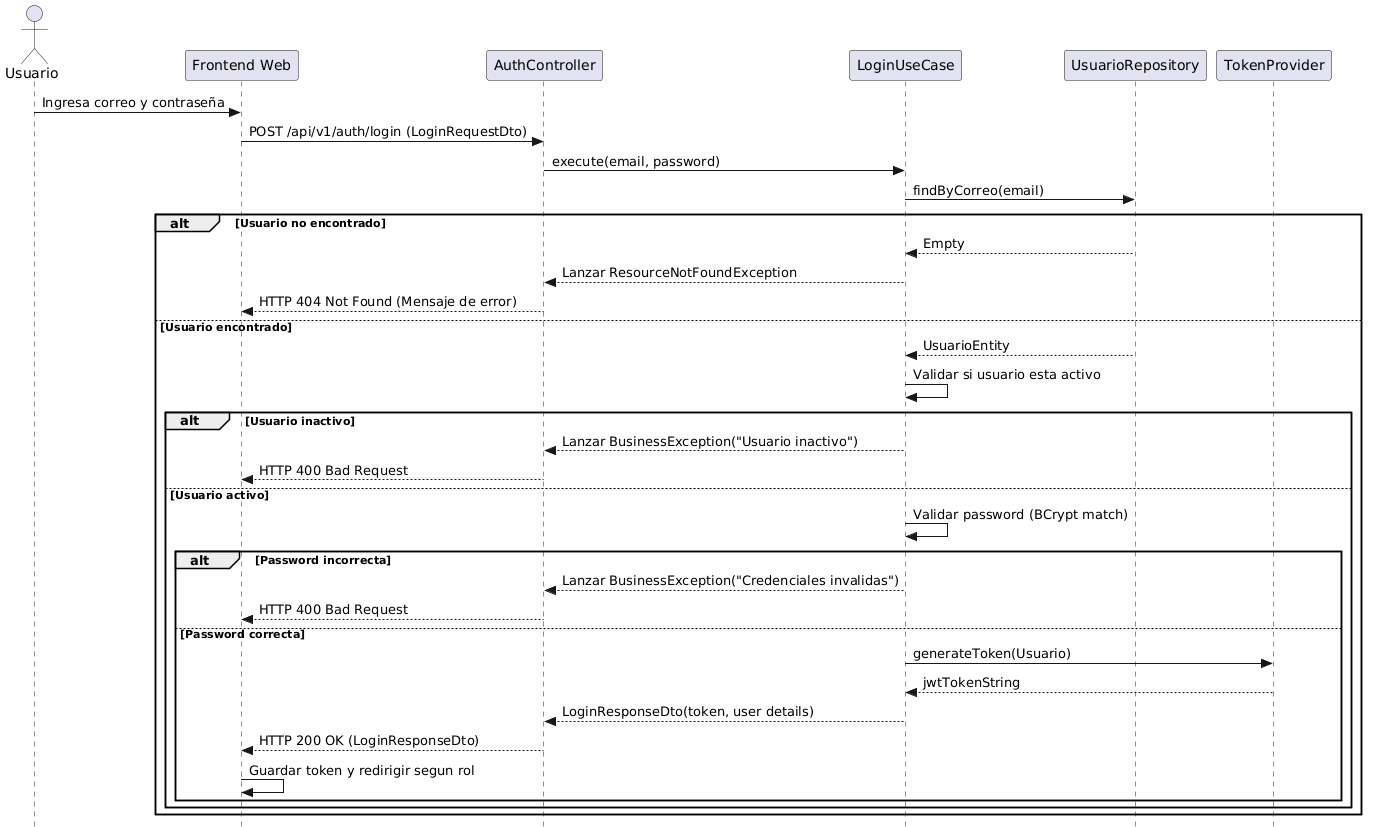
\includegraphics[width=0.9\textwidth]{login_local}
    \caption{Diagrama de secuencia del proceso de autenticación local y generación de JWT.}
    \label{fig:login_local}
\end{figure}

\subsection{Auto-registro de Estudiantes con Verificación por Correo}
El auto-registro de nuevos estudiantes o tesistas se gestiona mediante un flujo en dos pasos. El usuario envía sus datos iniciales (incluyendo su DNI, nombres, apellidos y correo institucional) al endpoint de registro. El sistema valida que el dominio del correo sea institucional (\texttt{.edu.pe}), verifica la inexistencia de duplicados en la base de datos y genera un código de verificación aleatorio de 6 dígitos que guarda temporalmente en memoria con un tiempo de expiración de 5 minutos.

En el segundo paso, el estudiante ingresa el código recibido en su correo electrónico. Si la clave temporal es válida y no ha expirado, el sistema cifra su contraseña con \texttt{BCrypt}, persiste su cuenta directamente en la base de datos física (asignándole el rol por defecto \texttt{ESTUDIANTE}), elimina los datos temporales en memoria y le provee un JWT firmado digitalmente para iniciar sesión de forma inmediata.

Este flujo de registro y verificación por código en memoria temporal se describe técnicamente en detalle en el archivo de especificación de flujos del sistema.

\subsection{Flujo de Cambio de Contraseña Obligatoria}
Para prevenir problemas de seguridad derivados del aprovisionamiento manual de cuentas por el administrador, el sistema exige que todos los usuarios que cuenten con inicio de sesión local cambien su contraseña por defecto al ingresar por primera vez. Si el indicador \texttt{must\_change\_password} está establecido en verdadero (\texttt{true}), el filtro de seguridad y el backend restringirán el acceso a los recursos comunes y guiarán al usuario hacia el formulario de actualización de contraseña. Tras un cambio exitoso, el indicador se establece en falso (\texttt{false}), liberando el acceso regular del usuario.

El flujo que rige la obligación de actualizar las credenciales locales de primer ingreso para mitigar riesgos de seguridad y desactivar el indicador de reinicio obligatorio se representa visualmente en la Figura~\ref{fig:cambio_password}.

\begin{figure}[htbp]
    \centering
    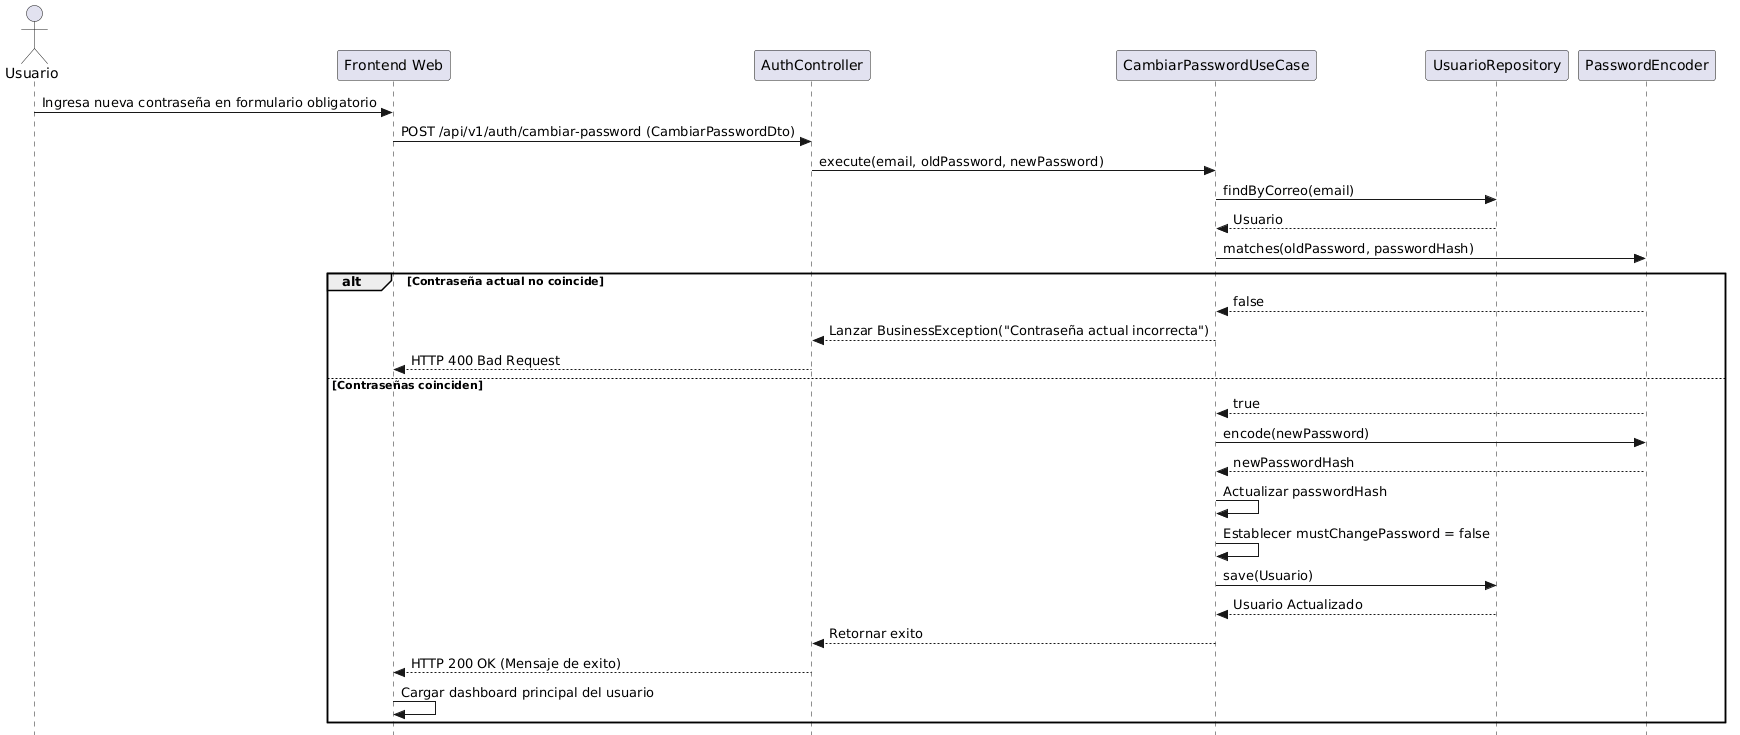
\includegraphics[width=0.85\textwidth]{cambio_password}
    \caption{Diagrama de secuencia de cambio obligatorio de contraseña en el primer inicio de sesión.}
    \label{fig:cambio_password}
\end{figure}

\subsection{Gestión de Usuarios y Creación de Cuentas}
El Administrador es el actor responsable de gestionar el ciclo de vida de los usuarios dentro del sistema. Al registrar un usuario, el caso de uso realiza validaciones de reglas de negocio: valida que el DNI no esté duplicado, que el correo institucional sea único y, en caso de no ingresarse un correo manualmente, el sistema genera automáticamente la dirección bajo el formato establecido por la regla institucional: \texttt{primer\_nombre.primer\_apellido@unas.edu.pe}.

Este flujo interactivo y las validaciones de duplicidad se representan de forma secuencial en la Figura~\ref{fig:crear_usuario}.

\begin{figure}[htbp]
    \centering
    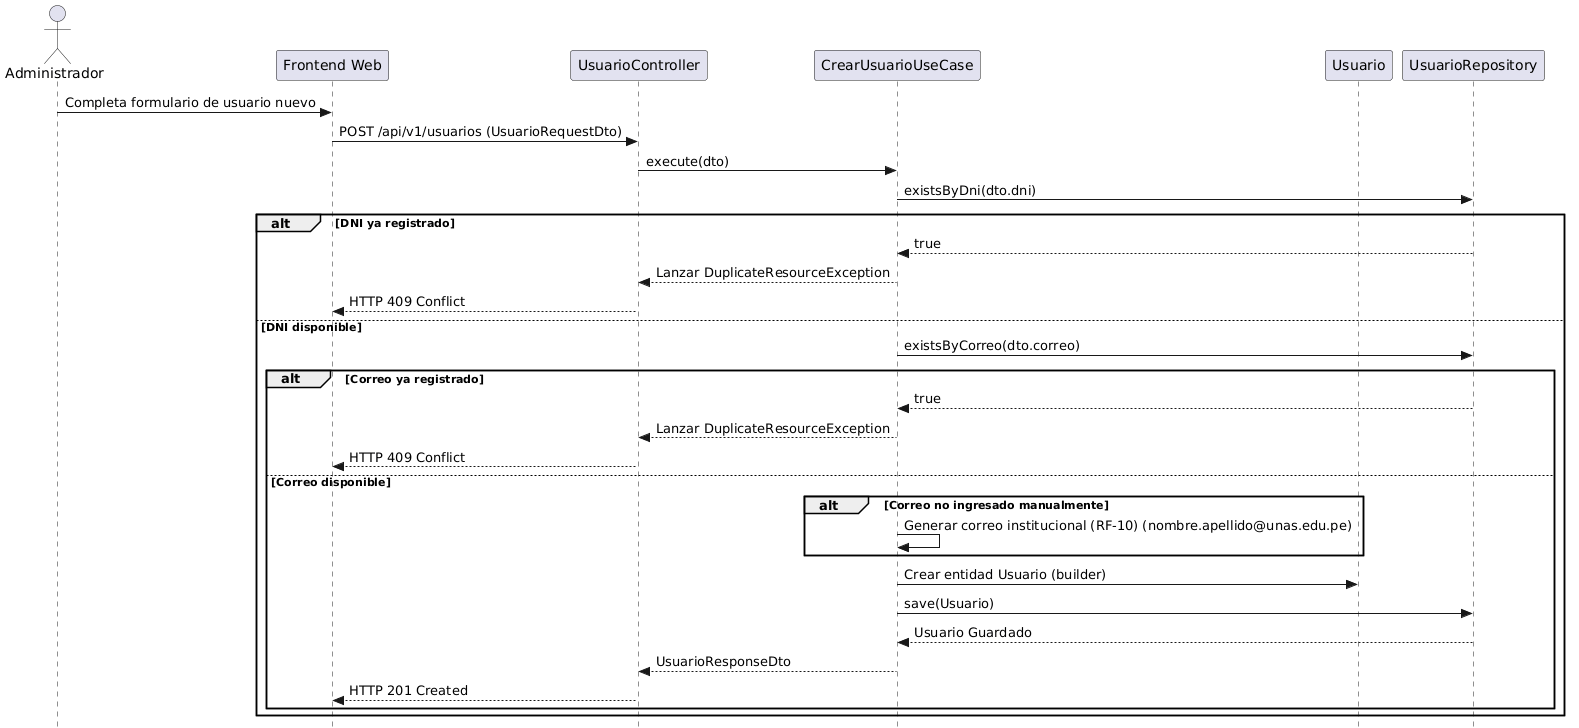
\includegraphics[width=0.9\textwidth]{crear_usuario}
    \caption{Diagrama de secuencia del proceso de creación y registro de usuarios por el Administrador.}
    \label{fig:crear_usuario}
\end{figure}

Además, la seguridad y el principio de mínimo privilegio en el sistema se gobiernan mediante una matriz de autorización detallada. Esta matriz define los permisos de los diferentes roles para cada uno de los endpoints de API críticos del módulo. Las políticas y privilegios correspondientes se estructuran formalmente en la Tabla~\ref{tab:control_acceso}.

\begin{table}[htbp]
\centering
\small
\resizebox{\textwidth}{!}{%
\begin{tabular}{|l|c|c|c|c|c|c|c|}
\hline
\textbf{API Endpoint / Recurso} & \textbf{ADM} & \textbf{EST} & \textbf{DOC} & \textbf{COOR} & \textbf{DIR} & \textbf{DEC} & \textbf{EVA} \\ \hline
\texttt{POST /api/v1/auth/login} & Permitir & Permitir & Permitir & Permitir & Permitir & Permitir & Permitir \\ \hline
\texttt{POST /api/v1/auth/change-password} & Permitir & Permitir & Permitir & Permitir & Permitir & Permitir & Permitir \\ \hline
\texttt{POST /api/v1/users} & Permitir & Denegar & Denegar & Denegar & Denegar & Denegar & Denegar \\ \hline
\texttt{GET /api/v1/users} & Permitir & Denegar & Denegar & Denegar & Denegar & Denegar & Denegar \\ \hline
\texttt{GET /api/v1/users/\{id\}} & Permitir & Denegar & Denegar & Denegar & Denegar & Denegar & Denegar \\ \hline
\texttt{PUT /api/v1/users/\{id\}} & Permitir & Denegar & Denegar & Denegar & Denegar & Denegar & Denegar \\ \hline
\texttt{PATCH /api/v1/users/\{id\}/status} & Permitir & Denegar & Denegar & Denegar & Denegar & Denegar & Denegar \\ \hline
\texttt{PATCH /api/v1/users/\{id\}/reset-password} & Permitir & Denegar & Denegar & Denegar & Denegar & Denegar & Denegar \\ \hline
\texttt{GET /api/v1/roles} & Permitir & Denegar & Denegar & Denegar & Denegar & Denegar & Denegar \\ \hline
\end{tabular}%
}
\caption{Matriz de control de acceso basada en roles (RBAC) para el módulo de seguridad (ADM: Administrador, EST: Estudiante, DOC: Docente Investigador, COOR: Coordinador, DIR: Director, DEC: Decano, EVA: Evaluador).}
\label{tab:control_acceso}
\end{table}

\newpage

% --- IMPLEMENTACIÓN TÉCNICA ---
\section{Detalles de Implementación Técnica}
La materialización del módulo en Spring Boot se rige por la estructuración de componentes desacoplados de infraestructura que operan en conjunto con los casos de uso definidos en la capa de aplicación.

\subsection{Filtro de Autenticación JWT}
El archivo \texttt{JwtAuthenticationFilter.java} hereda de \texttt{OncePerRequestFilter} para interceptar cada petición HTTP que entra al servidor. Se encarga de extraer la cabecera \texttt{Authorization}, extraer el token JWT, verificar su firma con la clave secreta y poblar el contexto de seguridad de Spring Security (\texttt{SecurityContextHolder}) si el token es válido. Esto permite aplicar directivas de seguridad a nivel de rutas y controladores de forma transparente.

\subsection{Configuración de Seguridad}
La configuración general de seguridad se define en \texttt{SecurityConfig.java}. Este componente acopla el soporte para tokens JWT locales, obligando a que toda comunicación REST sea completamente stateless. A continuación, se presenta este código:

\begin{lstlisting}[caption={Configuración de Spring Security para JWT.}]
package com.sgi.fiis.auth.infrastructure.security;

import org.springframework.context.annotation.Bean;
import org.springframework.context.annotation.Configuration;
import org.springframework.security.config.annotation.web.builders.HttpSecurity;
import org.springframework.security.config.annotation.web.configuration.EnableWebSecurity;
import org.springframework.security.config.http.SessionCreationPolicy;
import org.springframework.security.crypto.bcrypt.BCryptPasswordEncoder;
import org.springframework.security.crypto.password.PasswordEncoder;
import org.springframework.security.web.SecurityFilterChain;
import org.springframework.security.web.authentication.UsernamePasswordAuthenticationFilter;

@Configuration
@EnableWebSecurity
public class SecurityConfig {

    private final JwtAuthenticationFilter jwtAuthFilter;

    public SecurityConfig(JwtAuthenticationFilter jwtAuthFilter) {
        this.jwtAuthFilter = jwtAuthFilter;
    }

    @Bean
    public SecurityFilterChain securityFilterChain(HttpSecurity http) {
        try {
            http
                .csrf(csrf -> csrf.disable())
                .sessionManagement(session -> session.sessionCreationPolicy(SessionCreationPolicy.STATELESS))
                .authorizeHttpRequests(auth -> auth
                    .requestMatchers("/api/v1/auth/**").permitAll()
                    .requestMatchers("/health").permitAll()
                    .requestMatchers("/api/v1/users/**").hasRole("ADMIN")
                    .requestMatchers("/api/v1/roles/**").hasRole("ADMIN")
                    .anyRequest().authenticated()
                )
                .addFilterBefore(jwtAuthFilter, UsernamePasswordAuthenticationFilter.class)
                .exceptionHandling(exceptions -> exceptions
                    .defaultAuthenticationEntryPointFor(
                        new org.springframework.security.web.authentication.HttpStatusEntryPoint(org.springframework.http.HttpStatus.UNAUTHORIZED),
                        org.springframework.security.web.servlet.util.matcher.PathPatternRequestMatcher.pathPattern("/api/**")
                    )
                );

            return http.build();
        } catch (Exception e) {
            throw new IllegalStateException("Failed to configure security filter chain", e);
        }
    }

    @Bean
    public PasswordEncoder passwordEncoder() {
        return new BCryptPasswordEncoder();
    }
}
\end{lstlisting}

Esta configuración establece una arquitectura sin estado (\texttt{Stateless}) para todas las peticiones HTTP regulares que llevan cabeceras de autorización de tipo Bearer, eliminando completamente las sesiones en el servidor backend y disminuyendo riesgos de inyecciones y ataques CSRF.

\newpage

% --- CONCLUSIONES ---
\section{Conclusiones y Recomendaciones}
La construcción e implementación del módulo de seguridad para el SGI-FIIS aporta las siguientes conclusiones:
\begin{itemize}
    \item La adopción de la Arquitectura Limpia (Clean Architecture) reduce sustancialmente el acoplamiento del núcleo de la aplicación, facilitando la adición de futuros proveedores de identidad o cambios en el motor de base de datos sin afectar las reglas de negocio establecidas para los usuarios y los roles.
    \item El mecanismo de auto-registro local con verificación por código por correo institucional responde eficientemente al contexto universitario, promoviendo el aprovisionamiento automatizado y ágil de cuentas estudiantiles bajo un entorno de seguridad administrado.
    \item La inclusión del cambio de contraseña mandatorio y la deshabilitación lógica de cuentas en lugar de eliminaciones físicas garantizan la trazabilidad histórica de los trámites y proyectos en los cuales los usuarios participaron, mitigando riesgos de inconsistencia referencial en la base de datos del sistema de investigación.
\end{itemize}

Se recomienda implementar políticas rigurosas de expiración periódica de tokens JWT para fortalecer la integridad del sistema ante posibles fugas de credenciales locales en las terminales físicas de los usuarios de la facultad.

\newpage

% --- REFERENCIAS ---
\section{Referencias}
\begin{refcontext}
\begin{hangparas}{.5in}{1}
Beck, K. (2003). \textit{Test-Driven Development: By Example}. Addison-Wesley Professional.

Martin, R. C. (2018). \textit{Clean Architecture: A Craftsman's Guide to Software Structure and Design}. Prentice Hall.

% Referencia de Microsoft removida ya que se cambio a auto-registro local.

Spring Projects. (2026). \textit{Spring Security Reference}. VMware Tanzu. \url{https://docs.spring.io/spring-security/reference/}
\end{hangparas}
\end{refcontext}

\end{document}
